% Options for packages loaded elsewhere
\PassOptionsToPackage{unicode}{hyperref}
\PassOptionsToPackage{hyphens}{url}
%
\documentclass[
]{article}
\usepackage{lmodern}
\usepackage{amsmath}
\usepackage{ifxetex,ifluatex}
\ifnum 0\ifxetex 1\fi\ifluatex 1\fi=0 % if pdftex
  \usepackage[T1]{fontenc}
  \usepackage[utf8]{inputenc}
  \usepackage{textcomp} % provide euro and other symbols
  \usepackage{amssymb}
\else % if luatex or xetex
  \usepackage{unicode-math}
  \defaultfontfeatures{Scale=MatchLowercase}
  \defaultfontfeatures[\rmfamily]{Ligatures=TeX,Scale=1}
\fi
% Use upquote if available, for straight quotes in verbatim environments
\IfFileExists{upquote.sty}{\usepackage{upquote}}{}
\IfFileExists{microtype.sty}{% use microtype if available
  \usepackage[]{microtype}
  \UseMicrotypeSet[protrusion]{basicmath} % disable protrusion for tt fonts
}{}
\makeatletter
\@ifundefined{KOMAClassName}{% if non-KOMA class
  \IfFileExists{parskip.sty}{%
    \usepackage{parskip}
  }{% else
    \setlength{\parindent}{0pt}
    \setlength{\parskip}{6pt plus 2pt minus 1pt}}
}{% if KOMA class
  \KOMAoptions{parskip=half}}
\makeatother
\usepackage{xcolor}
\IfFileExists{xurl.sty}{\usepackage{xurl}}{} % add URL line breaks if available
\IfFileExists{bookmark.sty}{\usepackage{bookmark}}{\usepackage{hyperref}}
\hypersetup{
  pdftitle={Final Project- Background: Unionville Assets \& Challenges},
  pdfauthor={Will Finkelstein, MUP1.},
  hidelinks,
  pdfcreator={LaTeX via pandoc}}
\urlstyle{same} % disable monospaced font for URLs
\usepackage[margin=1in]{geometry}
\usepackage{color}
\usepackage{fancyvrb}
\newcommand{\VerbBar}{|}
\newcommand{\VERB}{\Verb[commandchars=\\\{\}]}
\DefineVerbatimEnvironment{Highlighting}{Verbatim}{commandchars=\\\{\}}
% Add ',fontsize=\small' for more characters per line
\usepackage{framed}
\definecolor{shadecolor}{RGB}{248,248,248}
\newenvironment{Shaded}{\begin{snugshade}}{\end{snugshade}}
\newcommand{\AlertTok}[1]{\textcolor[rgb]{0.94,0.16,0.16}{#1}}
\newcommand{\AnnotationTok}[1]{\textcolor[rgb]{0.56,0.35,0.01}{\textbf{\textit{#1}}}}
\newcommand{\AttributeTok}[1]{\textcolor[rgb]{0.77,0.63,0.00}{#1}}
\newcommand{\BaseNTok}[1]{\textcolor[rgb]{0.00,0.00,0.81}{#1}}
\newcommand{\BuiltInTok}[1]{#1}
\newcommand{\CharTok}[1]{\textcolor[rgb]{0.31,0.60,0.02}{#1}}
\newcommand{\CommentTok}[1]{\textcolor[rgb]{0.56,0.35,0.01}{\textit{#1}}}
\newcommand{\CommentVarTok}[1]{\textcolor[rgb]{0.56,0.35,0.01}{\textbf{\textit{#1}}}}
\newcommand{\ConstantTok}[1]{\textcolor[rgb]{0.00,0.00,0.00}{#1}}
\newcommand{\ControlFlowTok}[1]{\textcolor[rgb]{0.13,0.29,0.53}{\textbf{#1}}}
\newcommand{\DataTypeTok}[1]{\textcolor[rgb]{0.13,0.29,0.53}{#1}}
\newcommand{\DecValTok}[1]{\textcolor[rgb]{0.00,0.00,0.81}{#1}}
\newcommand{\DocumentationTok}[1]{\textcolor[rgb]{0.56,0.35,0.01}{\textbf{\textit{#1}}}}
\newcommand{\ErrorTok}[1]{\textcolor[rgb]{0.64,0.00,0.00}{\textbf{#1}}}
\newcommand{\ExtensionTok}[1]{#1}
\newcommand{\FloatTok}[1]{\textcolor[rgb]{0.00,0.00,0.81}{#1}}
\newcommand{\FunctionTok}[1]{\textcolor[rgb]{0.00,0.00,0.00}{#1}}
\newcommand{\ImportTok}[1]{#1}
\newcommand{\InformationTok}[1]{\textcolor[rgb]{0.56,0.35,0.01}{\textbf{\textit{#1}}}}
\newcommand{\KeywordTok}[1]{\textcolor[rgb]{0.13,0.29,0.53}{\textbf{#1}}}
\newcommand{\NormalTok}[1]{#1}
\newcommand{\OperatorTok}[1]{\textcolor[rgb]{0.81,0.36,0.00}{\textbf{#1}}}
\newcommand{\OtherTok}[1]{\textcolor[rgb]{0.56,0.35,0.01}{#1}}
\newcommand{\PreprocessorTok}[1]{\textcolor[rgb]{0.56,0.35,0.01}{\textit{#1}}}
\newcommand{\RegionMarkerTok}[1]{#1}
\newcommand{\SpecialCharTok}[1]{\textcolor[rgb]{0.00,0.00,0.00}{#1}}
\newcommand{\SpecialStringTok}[1]{\textcolor[rgb]{0.31,0.60,0.02}{#1}}
\newcommand{\StringTok}[1]{\textcolor[rgb]{0.31,0.60,0.02}{#1}}
\newcommand{\VariableTok}[1]{\textcolor[rgb]{0.00,0.00,0.00}{#1}}
\newcommand{\VerbatimStringTok}[1]{\textcolor[rgb]{0.31,0.60,0.02}{#1}}
\newcommand{\WarningTok}[1]{\textcolor[rgb]{0.56,0.35,0.01}{\textbf{\textit{#1}}}}
\usepackage{graphicx}
\makeatletter
\def\maxwidth{\ifdim\Gin@nat@width>\linewidth\linewidth\else\Gin@nat@width\fi}
\def\maxheight{\ifdim\Gin@nat@height>\textheight\textheight\else\Gin@nat@height\fi}
\makeatother
% Scale images if necessary, so that they will not overflow the page
% margins by default, and it is still possible to overwrite the defaults
% using explicit options in \includegraphics[width, height, ...]{}
\setkeys{Gin}{width=\maxwidth,height=\maxheight,keepaspectratio}
% Set default figure placement to htbp
\makeatletter
\def\fps@figure{htbp}
\makeatother
\setlength{\emergencystretch}{3em} % prevent overfull lines
\providecommand{\tightlist}{%
  \setlength{\itemsep}{0pt}\setlength{\parskip}{0pt}}
\setcounter{secnumdepth}{-\maxdimen} % remove section numbering
\ifluatex
  \usepackage{selnolig}  % disable illegal ligatures
\fi

\title{Final Project- Background: Unionville Assets \& Challenges}
\author{Will Finkelstein, MUP1.}
\date{4/02/2021}

\begin{document}
\maketitle

{
\setcounter{tocdepth}{2}
\tableofcontents
}
This RMD will provide an update of the more focused topic that will be
explored, along with some preliminary context that ties or compares
challenges in Unionville to those in other parts of Macon-Bibb County.

\#Context and Background

Unionville is a historically black, traditionally working class
neighborhood in the ``near west side'' of Macon. It is located just
across I-75 from Mercer University. Mercer has funded a lot of real
estate and foundational grant programs that spill into a few
``higher-need'' neighborhoods proximate to downtown, partially to permit
its continued development agenda. As Unionville is just outside of that
extended ``downtown'' area, the neighborhood is unable to access these.

Unionville has continued to transition from being a majority-homeowner
community to having a declining older homeowner, mostly renter
population. Children, having left long ago and having little interest in
holding onto their aging parents' homes, would sell these to any
interested buyer. This trend throughout the community has enabled
slumlords. Blight, illegal dumping, and high renter turnover have been
constant norms. Additionally, Unionville has had a reputation for gang
activity and violent crime since my early childhood. Without going too
deep into specific incidents, a significant number of last year's
shootings occurred close to hear. A number of neighborhood commercial
buildings have murals paying homage to community pillars who were
victims of gun violence. And the Bentley \& Sons Funeral Home, easily
its most renowned neighborhood institution, provides free services for
the families of victims as a social impact program. Yet, there are
stories of unity outside of struggle also. Former Mayor C. Jack Ellis,
Macon's first and only black mayor, began his civic career as a
community organizer in Unionville. The Frank Johnson Community Center,
operated by Parks \& Recreation, recently received around \$1 million
worth of renovations from SPLOST (Special Purpose Local Option Sales
Tax) revenues (Dunlap, 2017). The Macon-Bibb County Government's new
Public Works and Neighborhood Cleanup Collaborations consider Unionville
a major priority (Macon-Bibb County, 2021). And the neighborhood's
small, but strong business community takes a serious interest in seeing
the change happen.

The remainder of this background will discuss the spatial areas of
analysis (tracts and streets), the data sources in use, the analyses
that have already been and will be conducted, and the next steps for a
final product. While the initial plan was to conduct further analysis on
qualitative perspectives from long-term residents and neighborhood
leaders, some communication challenges with organizers and other time
constraints make that unfeasible at present. The expectations for how to
better engage the community will be in the form of an extension, briefly
described at the end.

\begin{Shaded}
\begin{Highlighting}[]
\FunctionTok{library}\NormalTok{(tidyverse)}
\end{Highlighting}
\end{Shaded}

\begin{verbatim}
## -- Attaching packages --------------------------------------- tidyverse 1.3.0 --
\end{verbatim}

\begin{verbatim}
## v ggplot2 3.3.3     v purrr   0.3.4
## v tibble  3.0.5     v dplyr   1.0.3
## v tidyr   1.1.2     v stringr 1.4.0
## v readr   1.4.0     v forcats 0.5.1
\end{verbatim}

\begin{verbatim}
## -- Conflicts ------------------------------------------ tidyverse_conflicts() --
## x dplyr::filter() masks stats::filter()
## x dplyr::lag()    masks stats::lag()
\end{verbatim}

\begin{Shaded}
\begin{Highlighting}[]
\FunctionTok{library}\NormalTok{(tidycensus)}
\FunctionTok{census\_api\_key}\NormalTok{(}\StringTok{"f6d3f308f00a0ffda3aa19e86807e0ea5960d86e"}\NormalTok{, }\AttributeTok{install =} \ConstantTok{TRUE}\NormalTok{, }\AttributeTok{overwrite=}\ConstantTok{TRUE}\NormalTok{) }
\end{Highlighting}
\end{Shaded}

\begin{verbatim}
## Your original .Renviron will be backed up and stored in your R HOME directory if needed.
\end{verbatim}

\begin{verbatim}
## Your API key has been stored in your .Renviron and can be accessed by Sys.getenv("CENSUS_API_KEY"). 
## To use now, restart R or run `readRenviron("~/.Renviron")`
\end{verbatim}

\begin{verbatim}
## [1] "f6d3f308f00a0ffda3aa19e86807e0ea5960d86e"
\end{verbatim}

\hypertarget{methods-and-approach}{%
\section{Methods and Approach}\label{methods-and-approach}}

For this ongoing project, I am conducting analyses that occur at three
spatial scales. One analysis occurs countywide, which evaluates the
relationship between ``Median Household Income'' and ``Proportion of
Population that is Black/African American'' in every census tract in
Bibb County, Georgia. This is at a single point in time, but draws the
picture of whether current sociodemographic data reflect trends
consistent with other places.A table and dot map will be included, with
each entry corresponding to a Census Tract. This is Macon-Bibb County's
location compared to the rest of Georgia, with interstates and larger
cities also highlighted:

\begin{Shaded}
\begin{Highlighting}[]
\NormalTok{knitr}\SpecialCharTok{::}\FunctionTok{include\_graphics}\NormalTok{(}\StringTok{"maconbibbonus.png"}\NormalTok{)}
\end{Highlighting}
\end{Shaded}

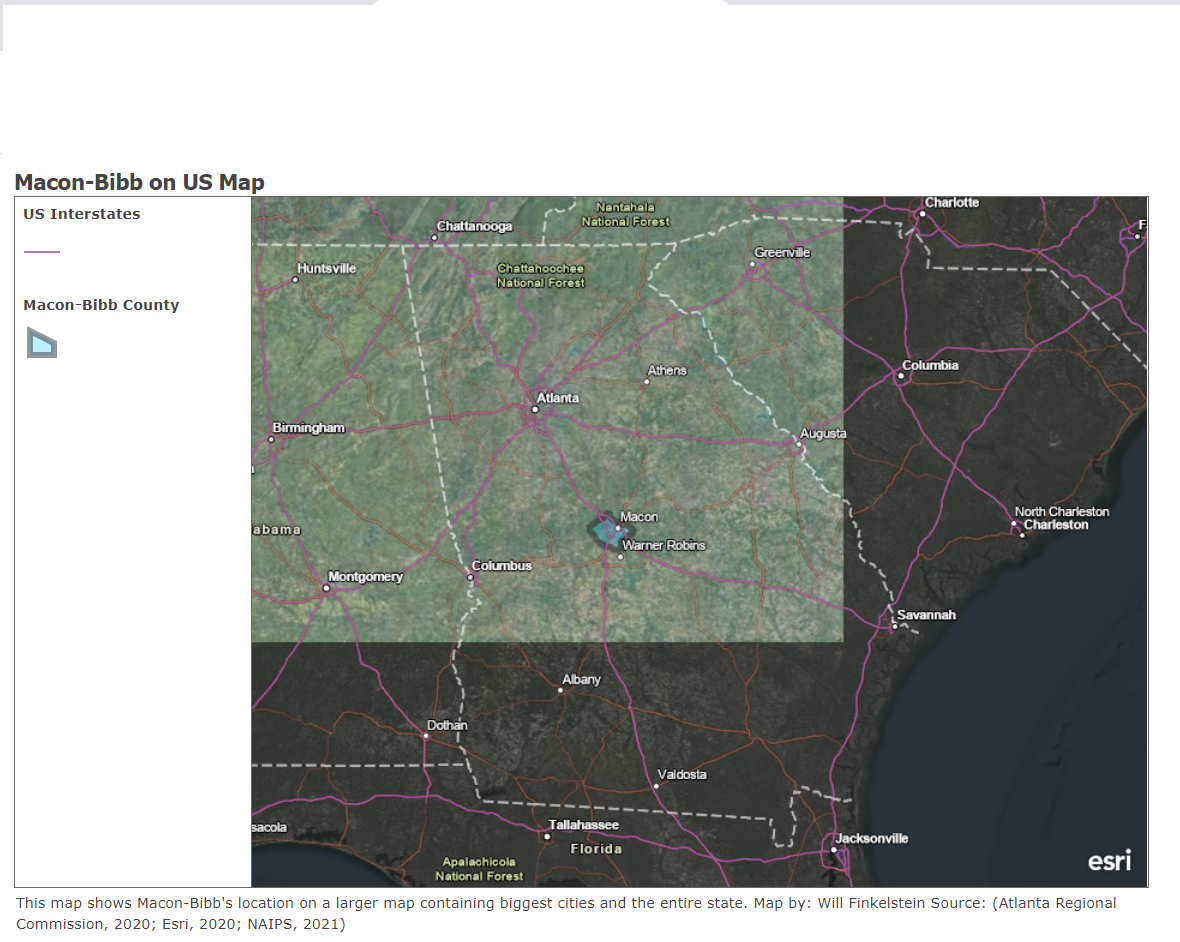
\includegraphics{maconbibbonus.png} There is some confusion about the
light intensity, but Macon-Bibb has been considered the fourth largest
community in Georgia since its 2014 consolidation. Compared to other
notable major cities, Macon-Bibb is located about 80 miles southeast of
Atlanta, 100 miles east of Columbus, 120 miles southwest of Augusta, 170
miles northwest of Savannah, and 90 miles southwest of Athens.

Next, Census Tract 104, which contains almost all of Unionville and a
couple of blocks of Napier Heights neighborhood, will be compared to two
other Census Tracts with similarities in sociodemographic
characteristics that are included within the general area that receives
investment from downtown specific programs. These are Census Tract 101,
which contains all of Macon's historic Pleasant Hill neighborhood
located right in the center of town, and Census Tract 138, located in
east Macon and including the neighborhoods of Mill Hill, Fort Hill, and
the Davis Homes Public Housing Development.Both of these border Macon's
central business district. Occupancy rates and median household incomes
are evaluated over a five year period (2015-19) for these three tracts,
to hopefully determine if connection to downtown investment
opportunities has begun to cause a revitalization.

\begin{Shaded}
\begin{Highlighting}[]
\NormalTok{knitr}\SpecialCharTok{::}\FunctionTok{include\_graphics}\NormalTok{(}\StringTok{"neighborhoodnalysiscomparativeareas.png"}\NormalTok{)}
\end{Highlighting}
\end{Shaded}

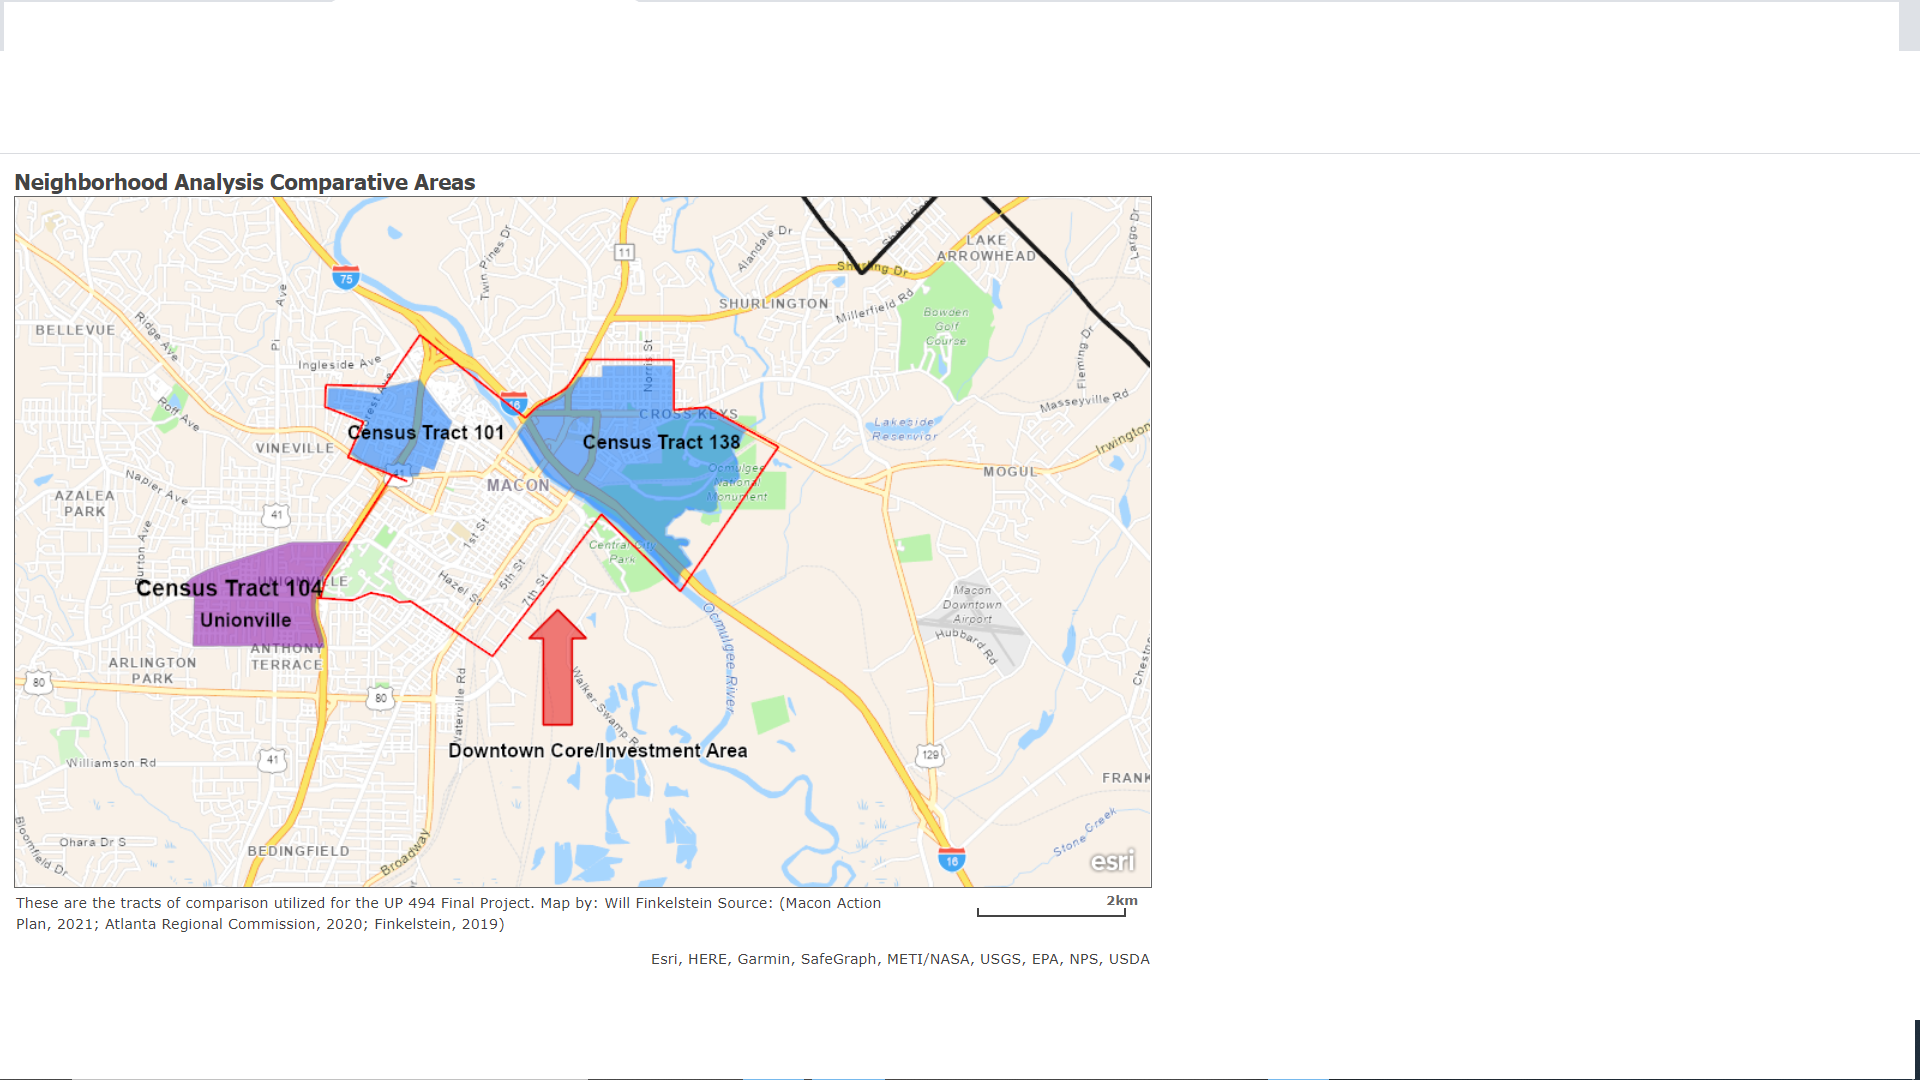
\includegraphics{neighborhoodnalysiscomparativeareas.png} The final
level of analysis occurs entirely in Census Tract 104. The plan is to
evaluate a potential relationship by road between Public Works
Department response times to reported property neglect and the number of
crimes to occur in 2020 on each road. The strongest precedent to the
work is consistent reporting that a clear majority of Macon-Bibb's
record breaking 51 homicides occurred in Unionville (Hicks, 2020). The
following map visualizes Census Tract 104 close up, also indicating
built barriers (interstate, university) that separate this from the
larger area considered downtown:

\begin{Shaded}
\begin{Highlighting}[]
\NormalTok{knitr}\SpecialCharTok{::}\FunctionTok{include\_graphics}\NormalTok{(}\StringTok{"unionvillemap.png"}\NormalTok{)}
\end{Highlighting}
\end{Shaded}

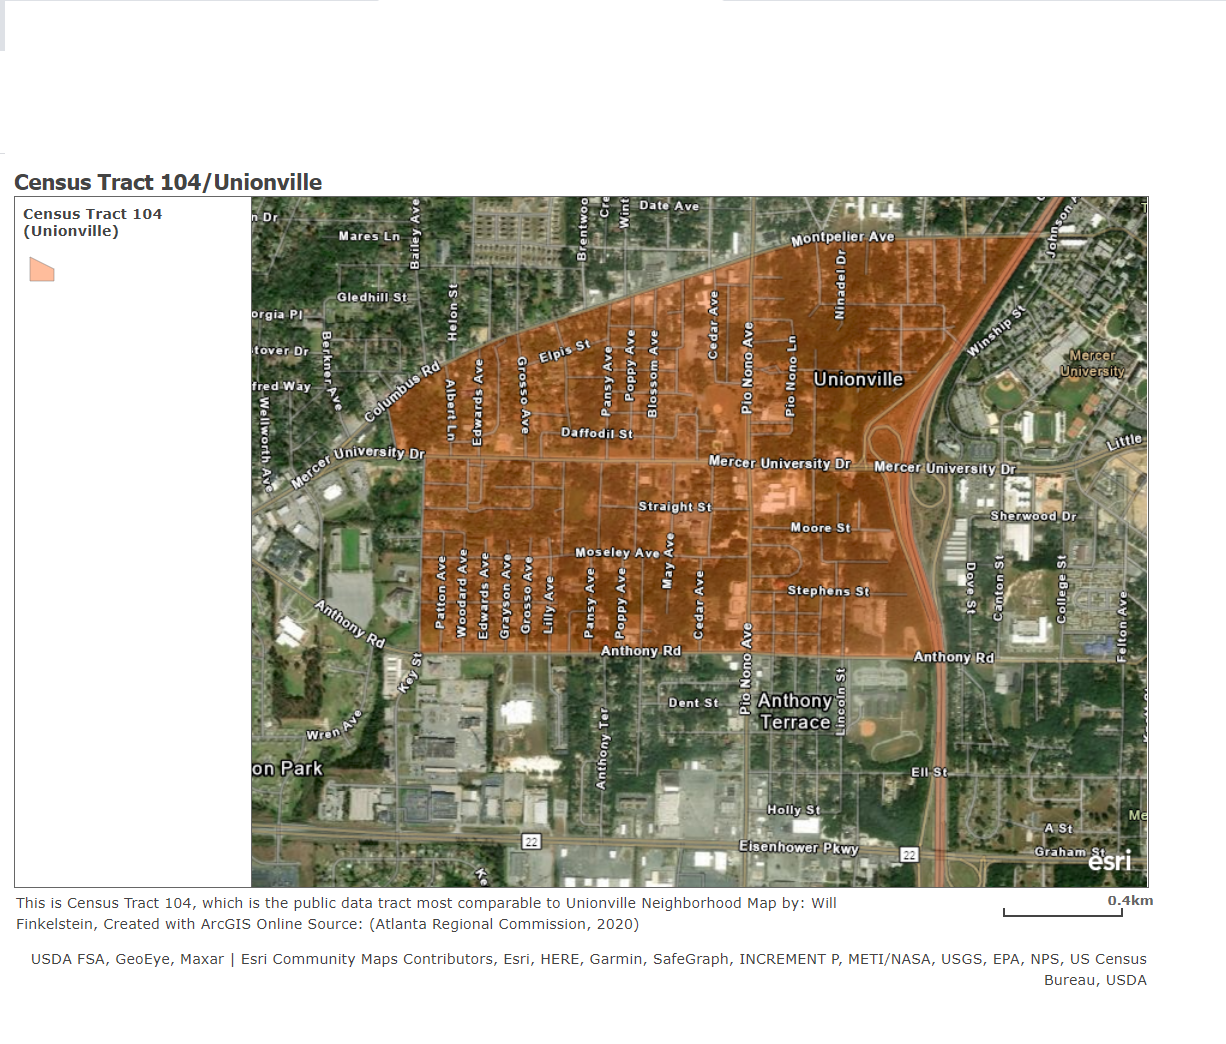
\includegraphics{unionvillemap.png} The data is still in process for
this. But after evaluating these at the street level, tract-wide
response times to crime rates may be compared with Tracts 101 and 138 as
well.

\hypertarget{data-sources}{%
\section{Data Sources}\label{data-sources}}

The county wide and three tract comparative analyses rely on ACS 5 year
data from the US census Bureau. These include Table B19013 (Median
Household Income), Table B02001 (Race), and Table DP04 (Housing
Characteristics) for years 2015, 2016, 2017, 2018, 2019. After importing
selected variables, values are added using mutate for certain variables
such as year and percentage black.

While this data request is still in process, data for the final street
by street analysis in Census Tract 104 will utilize sets imported from
agencies within the combined Macon-Bibb County government. Crime data
for 2020 will come from the ``highly understaffed'' Bibb County
Sheriff's office and property neglect data will come from the county's
license with ``SeeClickFix''. ``SeeClickFix'' allows residents to report
instances of property neglect, lack of code enforcement, illegal
dumping, and various other situations of public neglect. Complaints go
into the potential scopes of eight government departments. These are
Solid Waste and its privatized partner for residential trash disposal
(ADS), Traffic, Recreation, Public Works, Facilities Management, Code
Enforcement, Animal Services, Beautification (MaconBibb.us, 2021).

\#Preliminary Analysis While continuing to wait for local data, I went
ahead and utilized Census data to contact county-wide and three tract
comparisons.

After running code and plotting the relationship between ``Median
Household Income'' and ``Proportion of Population that is Black/African
American'' in every census tract in Bibb County, Georgia, I got the
following table:

\begin{Shaded}
\begin{Highlighting}[]
\NormalTok{maconbibbmhi\_2019 }\OtherTok{\textless{}{-}} \FunctionTok{get\_acs}\NormalTok{(}\AttributeTok{geography =} \StringTok{"tract"}\NormalTok{, }\AttributeTok{state =} \StringTok{"GA"}\NormalTok{, }\AttributeTok{county =} \StringTok{"Bibb"}\NormalTok{, }\AttributeTok{table =} \StringTok{"B19013"}\NormalTok{, }\AttributeTok{year=}\DecValTok{2019}\NormalTok{, }\AttributeTok{survey=}\StringTok{"acs5"}\NormalTok{, }\AttributeTok{output=}\StringTok{"wide"}\NormalTok{) }\SpecialCharTok{\%\textgreater{}\%}
\FunctionTok{select}\NormalTok{(NAME, B19013\_001E) }\SpecialCharTok{\%\textgreater{}\%}
\FunctionTok{rename}\NormalTok{(}\AttributeTok{Neighborhood =}\NormalTok{ NAME, }\AttributeTok{mhi =}\NormalTok{ B19013\_001E) }
\end{Highlighting}
\end{Shaded}

\begin{verbatim}
## Getting data from the 2015-2019 5-year ACS
\end{verbatim}

\begin{verbatim}
## Loading ACS5 variables for 2019 from table B19013. To cache this dataset for faster access to ACS tables in the future, run this function with `cache_table = TRUE`. You only need to do this once per ACS dataset.
\end{verbatim}

\begin{Shaded}
\begin{Highlighting}[]
\NormalTok{maconbibbmhi\_2019 }
\end{Highlighting}
\end{Shaded}

\begin{verbatim}
## # A tibble: 44 x 2
##    Neighborhood                                mhi
##    <chr>                                     <dbl>
##  1 Census Tract 135.04, Bibb County, Georgia 69118
##  2 Census Tract 136.03, Bibb County, Georgia 66996
##  3 Census Tract 136.04, Bibb County, Georgia 55000
##  4 Census Tract 136.05, Bibb County, Georgia 70379
##  5 Census Tract 136.06, Bibb County, Georgia 77143
##  6 Census Tract 137, Bibb County, Georgia    22439
##  7 Census Tract 138, Bibb County, Georgia    19063
##  8 Census Tract 139, Bibb County, Georgia    34261
##  9 Census Tract 135.02, Bibb County, Georgia 41523
## 10 Census Tract 123, Bibb County, Georgia    21205
## # ... with 34 more rows
\end{verbatim}

\begin{Shaded}
\begin{Highlighting}[]
\NormalTok{maconbibb\_blackpopulation\_2019 }\OtherTok{\textless{}{-}}\FunctionTok{get\_acs}\NormalTok{(}\AttributeTok{geography =} \StringTok{"tract"}\NormalTok{, }\AttributeTok{state =} \StringTok{"GA"}\NormalTok{,}\AttributeTok{county =} \StringTok{"Bibb"}\NormalTok{, }\AttributeTok{table =} \StringTok{"B02001"}\NormalTok{, }\AttributeTok{year=}\DecValTok{2019}\NormalTok{, }\AttributeTok{survey=}\StringTok{"acs5"}\NormalTok{, }\AttributeTok{output=}\StringTok{"wide"}\NormalTok{) }\SpecialCharTok{\%\textgreater{}\%} 
\FunctionTok{rename}\NormalTok{(}\AttributeTok{Neighborhood =}\NormalTok{ NAME,}
       \AttributeTok{pop\_tot=}\NormalTok{ B02001\_001E,}
       \AttributeTok{pop\_black =}\NormalTok{ B02001\_003E) }\SpecialCharTok{\%\textgreater{}\%}
 \FunctionTok{select}\NormalTok{(Neighborhood, pop\_tot, pop\_black) }\SpecialCharTok{\%\textgreater{}\%}
 \FunctionTok{mutate}\NormalTok{(}\AttributeTok{p\_black =}\NormalTok{ pop\_black}\SpecialCharTok{/}\NormalTok{pop\_tot) }\SpecialCharTok{\%\textgreater{}\%}
 \FunctionTok{select}\NormalTok{(Neighborhood, p\_black)}
\end{Highlighting}
\end{Shaded}

\begin{verbatim}
## Getting data from the 2015-2019 5-year ACS
\end{verbatim}

\begin{verbatim}
## Loading ACS5 variables for 2019 from table B02001. To cache this dataset for faster access to ACS tables in the future, run this function with `cache_table = TRUE`. You only need to do this once per ACS dataset.
\end{verbatim}

\begin{Shaded}
\begin{Highlighting}[]
\NormalTok{maconbibb\_blackpopulation\_2019}
\end{Highlighting}
\end{Shaded}

\begin{verbatim}
## # A tibble: 44 x 2
##    Neighborhood                              p_black
##    <chr>                                       <dbl>
##  1 Census Tract 135.04, Bibb County, Georgia   0.251
##  2 Census Tract 136.03, Bibb County, Georgia   0.339
##  3 Census Tract 136.04, Bibb County, Georgia   0.339
##  4 Census Tract 136.05, Bibb County, Georgia   0.555
##  5 Census Tract 136.06, Bibb County, Georgia   0.337
##  6 Census Tract 137, Bibb County, Georgia      0.585
##  7 Census Tract 138, Bibb County, Georgia      0.946
##  8 Census Tract 139, Bibb County, Georgia      0.464
##  9 Census Tract 135.02, Bibb County, Georgia   0.184
## 10 Census Tract 123, Bibb County, Georgia      0.775
## # ... with 34 more rows
\end{verbatim}

\begin{Shaded}
\begin{Highlighting}[]
\NormalTok{NeighborhoodIncomeRace }\OtherTok{\textless{}{-}} \FunctionTok{bind\_cols}\NormalTok{(maconbibbmhi\_2019, maconbibb\_blackpopulation\_2019) }\SpecialCharTok{\%\textgreater{}\%} 
 \FunctionTok{rename}\NormalTok{(}\AttributeTok{Neighborhood =}\NormalTok{ Neighborhood...}\DecValTok{1}\NormalTok{) }\SpecialCharTok{\%\textgreater{}\%}
 \FunctionTok{select}\NormalTok{(Neighborhood, mhi, p\_black) }
\end{Highlighting}
\end{Shaded}

\begin{verbatim}
## New names:
## * Neighborhood -> Neighborhood...1
## * Neighborhood -> Neighborhood...3
\end{verbatim}

\begin{Shaded}
\begin{Highlighting}[]
\NormalTok{NeighborhoodIncomeRace}
\end{Highlighting}
\end{Shaded}

\begin{verbatim}
## # A tibble: 44 x 3
##    Neighborhood                                mhi p_black
##    <chr>                                     <dbl>   <dbl>
##  1 Census Tract 135.04, Bibb County, Georgia 69118   0.251
##  2 Census Tract 136.03, Bibb County, Georgia 66996   0.339
##  3 Census Tract 136.04, Bibb County, Georgia 55000   0.339
##  4 Census Tract 136.05, Bibb County, Georgia 70379   0.555
##  5 Census Tract 136.06, Bibb County, Georgia 77143   0.337
##  6 Census Tract 137, Bibb County, Georgia    22439   0.585
##  7 Census Tract 138, Bibb County, Georgia    19063   0.946
##  8 Census Tract 139, Bibb County, Georgia    34261   0.464
##  9 Census Tract 135.02, Bibb County, Georgia 41523   0.184
## 10 Census Tract 123, Bibb County, Georgia    21205   0.775
## # ... with 34 more rows
\end{verbatim}

The table was then adapted into a dot plot:

\begin{Shaded}
\begin{Highlighting}[]
\NormalTok{macontract\_mhi\_race }\OtherTok{\textless{}{-}} \FunctionTok{ggplot}\NormalTok{(NeighborhoodIncomeRace, }\FunctionTok{aes}\NormalTok{(p\_black, mhi)) }\SpecialCharTok{+} \FunctionTok{geom\_point}\NormalTok{(}\AttributeTok{color =} \StringTok{"blue"}\NormalTok{) }\SpecialCharTok{+} 
\FunctionTok{scale\_x\_log10}\NormalTok{(}\AttributeTok{labels =}\NormalTok{ scales}\SpecialCharTok{::}\NormalTok{percent) }\SpecialCharTok{+}
\FunctionTok{scale\_y\_log10}\NormalTok{(}\AttributeTok{labels =}\NormalTok{ scales}\SpecialCharTok{::}\NormalTok{dollar) }\SpecialCharTok{+} 
\FunctionTok{labs}\NormalTok{(}\AttributeTok{x =} \StringTok{"Percentage Black by Census Tract"}\NormalTok{, }\AttributeTok{y =} \StringTok{"Median Household Income"}\NormalTok{,}
     \AttributeTok{title =} \StringTok{"Median Household Income by Proportion of Population{-}Black"}\NormalTok{,}
     \AttributeTok{subtitle =}  \StringTok{"Ordered by Census Tract in Macon{-}Bibb County, Based on 2019 ACS 5 yr Estimates"}\NormalTok{,}
     \AttributeTok{caption =} \StringTok{"Source: (US Census Bureau, 2020)"}\NormalTok{)}
\NormalTok{macontract\_mhi\_race}
\end{Highlighting}
\end{Shaded}

\includegraphics{UP494FinalProjectBackground_UnionvilleAssetChallengeInventory_willfinkelstein_files/figure-latex/unnamed-chunk-6-1.pdf}
With the exception of one tract, which contains Mercer University and
benefits from the Census' counting of students as low income
individuals, every other tract in the low income category
(\textless\$30,000 for this context) is majority black. The highest
income tract, 134.10, is only 12\% black. It has a median household
income of \$91,116. Only one majority-black tract, 136.05, out of the 25
that are over half black has a median household income over \$40,000.
Its median household income is \$70,379. This demonstrates a high level
of inequality and presumed segregation, a consistent characteristic in
majority-minority communities.

A longitudinal comparison of the median household incomes in Tracts 101,
104, and 138 is tabulated with the following code:

\begin{Shaded}
\begin{Highlighting}[]
\NormalTok{areasmhi19 }\OtherTok{\textless{}{-}} \FunctionTok{get\_acs}\NormalTok{(}\AttributeTok{geography =} \StringTok{"tract"}\NormalTok{, }\AttributeTok{state =} \StringTok{"GA"}\NormalTok{, }\AttributeTok{county =} \StringTok{"Bibb"}\NormalTok{, }\AttributeTok{table =} \StringTok{"B19013"}\NormalTok{, }\AttributeTok{year=}\DecValTok{2019}\NormalTok{, }\AttributeTok{survey=}\StringTok{"acs5"}\NormalTok{, }\AttributeTok{output=}\StringTok{"wide"}\NormalTok{)}\SpecialCharTok{\%\textgreater{}\%}
\FunctionTok{filter}\NormalTok{(NAME }\SpecialCharTok{\%in\%} \FunctionTok{c}\NormalTok{(}\StringTok{"Census Tract 101, Bibb County, Georgia"}\NormalTok{, }\StringTok{"Census Tract 104, Bibb County, Georgia"}\NormalTok{, }\StringTok{"Census Tract 138, Bibb County, Georgia"}\NormalTok{)) }\SpecialCharTok{\%\textgreater{}\%}
\FunctionTok{mutate}\NormalTok{(}\AttributeTok{year =} \FunctionTok{case\_when}\NormalTok{(}
\NormalTok{  B19013\_001M }\SpecialCharTok{==} \StringTok{"8942"} \SpecialCharTok{\textasciitilde{}} \StringTok{"2019"}\NormalTok{,}
\NormalTok{  B19013\_001M }\SpecialCharTok{==} \StringTok{"4274"} \SpecialCharTok{\textasciitilde{}} \StringTok{"2019"}\NormalTok{,}
\NormalTok{  B19013\_001M }\SpecialCharTok{==} \StringTok{"7423"} \SpecialCharTok{\textasciitilde{}} \StringTok{"2019"}\NormalTok{) ) }\SpecialCharTok{\%\textgreater{}\%}
\FunctionTok{select}\NormalTok{(NAME, B19013\_001E, year) }\SpecialCharTok{\%\textgreater{}\%}
\FunctionTok{rename}\NormalTok{(}\AttributeTok{neighborhood =}\NormalTok{ NAME, }\AttributeTok{mhi =}\NormalTok{ B19013\_001E) }
\end{Highlighting}
\end{Shaded}

\begin{verbatim}
## Getting data from the 2015-2019 5-year ACS
\end{verbatim}

\begin{verbatim}
## Loading ACS5 variables for 2019 from table B19013. To cache this dataset for faster access to ACS tables in the future, run this function with `cache_table = TRUE`. You only need to do this once per ACS dataset.
\end{verbatim}

\begin{Shaded}
\begin{Highlighting}[]
\NormalTok{areasmhi18 }\OtherTok{\textless{}{-}} \FunctionTok{get\_acs}\NormalTok{(}\AttributeTok{geography =} \StringTok{"tract"}\NormalTok{, }\AttributeTok{state =} \StringTok{"GA"}\NormalTok{, }\AttributeTok{county =} \StringTok{"Bibb"}\NormalTok{, }\AttributeTok{table =} \StringTok{"B19013"}\NormalTok{, }\AttributeTok{year=}\DecValTok{2018}\NormalTok{, }\AttributeTok{survey=}\StringTok{"acs5"}\NormalTok{, }\AttributeTok{output=}\StringTok{"wide"}\NormalTok{)}\SpecialCharTok{\%\textgreater{}\%}
\FunctionTok{filter}\NormalTok{(NAME }\SpecialCharTok{\%in\%} \FunctionTok{c}\NormalTok{(}\StringTok{"Census Tract 101, Bibb County, Georgia"}\NormalTok{, }\StringTok{"Census Tract 104, Bibb County, Georgia"}\NormalTok{, }\StringTok{"Census Tract 138, Bibb County, Georgia"}\NormalTok{)) }\SpecialCharTok{\%\textgreater{}\%}
\FunctionTok{mutate}\NormalTok{(}\AttributeTok{year =} \FunctionTok{case\_when}\NormalTok{(}
\NormalTok{  B19013\_001M }\SpecialCharTok{==} \StringTok{"9704"} \SpecialCharTok{\textasciitilde{}} \StringTok{"2018"}\NormalTok{,}
\NormalTok{  B19013\_001M }\SpecialCharTok{==} \StringTok{"6460"} \SpecialCharTok{\textasciitilde{}} \StringTok{"2018"}\NormalTok{,}
\NormalTok{  B19013\_001M }\SpecialCharTok{==} \StringTok{"4280"} \SpecialCharTok{\textasciitilde{}} \StringTok{"2018"}\NormalTok{) ) }\SpecialCharTok{\%\textgreater{}\%}
\FunctionTok{select}\NormalTok{(NAME, B19013\_001E, year) }\SpecialCharTok{\%\textgreater{}\%}
\FunctionTok{rename}\NormalTok{(}\AttributeTok{neighborhood =}\NormalTok{ NAME, }\AttributeTok{mhi =}\NormalTok{ B19013\_001E) }
\end{Highlighting}
\end{Shaded}

\begin{verbatim}
## Getting data from the 2014-2018 5-year ACS
\end{verbatim}

\begin{verbatim}
## Loading ACS5 variables for 2018 from table B19013. To cache this dataset for faster access to ACS tables in the future, run this function with `cache_table = TRUE`. You only need to do this once per ACS dataset.
\end{verbatim}

\begin{Shaded}
\begin{Highlighting}[]
\NormalTok{areasmhi17 }\OtherTok{\textless{}{-}} \FunctionTok{get\_acs}\NormalTok{(}\AttributeTok{geography =} \StringTok{"tract"}\NormalTok{, }\AttributeTok{state =} \StringTok{"GA"}\NormalTok{, }\AttributeTok{county =} \StringTok{"Bibb"}\NormalTok{, }\AttributeTok{table =} \StringTok{"B19013"}\NormalTok{, }\AttributeTok{year=}\DecValTok{2017}\NormalTok{, }\AttributeTok{survey=}\StringTok{"acs5"}\NormalTok{, }\AttributeTok{output=}\StringTok{"wide"}\NormalTok{) }\SpecialCharTok{\%\textgreater{}\%}
\FunctionTok{filter}\NormalTok{(NAME }\SpecialCharTok{\%in\%} \FunctionTok{c}\NormalTok{(}\StringTok{"Census Tract 101, Bibb County, Georgia"}\NormalTok{, }\StringTok{"Census Tract 104, Bibb County, Georgia"}\NormalTok{, }\StringTok{"Census Tract 138, Bibb County, Georgia"}\NormalTok{)) }\SpecialCharTok{\%\textgreater{}\%}
\FunctionTok{mutate}\NormalTok{(}\AttributeTok{year =} \FunctionTok{case\_when}\NormalTok{(}
\NormalTok{  B19013\_001M }\SpecialCharTok{==} \StringTok{"5841"} \SpecialCharTok{\textasciitilde{}} \StringTok{"2017"}\NormalTok{,}
\NormalTok{  B19013\_001M }\SpecialCharTok{==} \StringTok{"7934"} \SpecialCharTok{\textasciitilde{}} \StringTok{"2017"}\NormalTok{,}
\NormalTok{  B19013\_001M }\SpecialCharTok{==} \StringTok{"6285"} \SpecialCharTok{\textasciitilde{}} \StringTok{"2017"}\NormalTok{) ) }\SpecialCharTok{\%\textgreater{}\%}
\FunctionTok{select}\NormalTok{(NAME, B19013\_001E, year) }\SpecialCharTok{\%\textgreater{}\%}
\FunctionTok{rename}\NormalTok{(}\AttributeTok{neighborhood =}\NormalTok{ NAME, }\AttributeTok{mhi =}\NormalTok{ B19013\_001E)}
\end{Highlighting}
\end{Shaded}

\begin{verbatim}
## Getting data from the 2013-2017 5-year ACS
\end{verbatim}

\begin{verbatim}
## Loading ACS5 variables for 2017 from table B19013. To cache this dataset for faster access to ACS tables in the future, run this function with `cache_table = TRUE`. You only need to do this once per ACS dataset.
\end{verbatim}

\begin{Shaded}
\begin{Highlighting}[]
\NormalTok{areasmhi16 }\OtherTok{\textless{}{-}} \FunctionTok{get\_acs}\NormalTok{(}\AttributeTok{geography =} \StringTok{"tract"}\NormalTok{, }\AttributeTok{state =} \StringTok{"GA"}\NormalTok{, }\AttributeTok{county =} \StringTok{"Bibb"}\NormalTok{, }\AttributeTok{table =} \StringTok{"B19013"}\NormalTok{, }\AttributeTok{year=}\DecValTok{2016}\NormalTok{, }\AttributeTok{survey=}\StringTok{"acs5"}\NormalTok{, }\AttributeTok{output=}\StringTok{"wide"}\NormalTok{) }\SpecialCharTok{\%\textgreater{}\%}
\FunctionTok{filter}\NormalTok{(NAME }\SpecialCharTok{\%in\%} \FunctionTok{c}\NormalTok{(}\StringTok{"Census Tract 101, Bibb County, Georgia"}\NormalTok{, }\StringTok{"Census Tract 104, Bibb County, Georgia"}\NormalTok{, }\StringTok{"Census Tract 138, Bibb County, Georgia"}\NormalTok{)) }\SpecialCharTok{\%\textgreater{}\%}
\FunctionTok{mutate}\NormalTok{(}\AttributeTok{year =} \FunctionTok{case\_when}\NormalTok{(}
\NormalTok{  B19013\_001M }\SpecialCharTok{==} \StringTok{"5466"} \SpecialCharTok{\textasciitilde{}} \StringTok{"2016"}\NormalTok{,}
\NormalTok{  B19013\_001M }\SpecialCharTok{==} \StringTok{"8125"} \SpecialCharTok{\textasciitilde{}} \StringTok{"2016"}\NormalTok{,}
\NormalTok{  B19013\_001M }\SpecialCharTok{==} \StringTok{"4597"} \SpecialCharTok{\textasciitilde{}} \StringTok{"2016"}\NormalTok{) ) }\SpecialCharTok{\%\textgreater{}\%}
\FunctionTok{select}\NormalTok{(NAME, B19013\_001E, year) }\SpecialCharTok{\%\textgreater{}\%}
\FunctionTok{rename}\NormalTok{(}\AttributeTok{neighborhood =}\NormalTok{ NAME, }\AttributeTok{mhi =}\NormalTok{ B19013\_001E)}
\end{Highlighting}
\end{Shaded}

\begin{verbatim}
## Getting data from the 2012-2016 5-year ACS
\end{verbatim}

\begin{verbatim}
## Loading ACS5 variables for 2016 from table B19013. To cache this dataset for faster access to ACS tables in the future, run this function with `cache_table = TRUE`. You only need to do this once per ACS dataset.
\end{verbatim}

\begin{Shaded}
\begin{Highlighting}[]
\NormalTok{areasmhi15 }\OtherTok{\textless{}{-}} \FunctionTok{get\_acs}\NormalTok{(}\AttributeTok{geography =} \StringTok{"tract"}\NormalTok{, }\AttributeTok{state =} \StringTok{"GA"}\NormalTok{, }\AttributeTok{county =} \StringTok{"Bibb"}\NormalTok{, }\AttributeTok{table =} \StringTok{"B19013"}\NormalTok{, }\AttributeTok{year=}\DecValTok{2015}\NormalTok{, }\AttributeTok{survey=}\StringTok{"acs5"}\NormalTok{, }\AttributeTok{output=}\StringTok{"wide"}\NormalTok{) }\SpecialCharTok{\%\textgreater{}\%}
\FunctionTok{filter}\NormalTok{(NAME }\SpecialCharTok{\%in\%} \FunctionTok{c}\NormalTok{(}\StringTok{"Census Tract 101, Bibb County, Georgia"}\NormalTok{, }\StringTok{"Census Tract 104, Bibb County, Georgia"}\NormalTok{, }\StringTok{"Census Tract 138, Bibb County, Georgia"}\NormalTok{)) }\SpecialCharTok{\%\textgreater{}\%}
\FunctionTok{mutate}\NormalTok{(}\AttributeTok{year =} \FunctionTok{case\_when}\NormalTok{(}
\NormalTok{  B19013\_001M }\SpecialCharTok{==} \StringTok{"4935"} \SpecialCharTok{\textasciitilde{}} \StringTok{"2015"}\NormalTok{,}
\NormalTok{  B19013\_001M }\SpecialCharTok{==} \StringTok{"2629"} \SpecialCharTok{\textasciitilde{}} \StringTok{"2015"}\NormalTok{,}
\NormalTok{  B19013\_001M }\SpecialCharTok{==} \StringTok{"4138"} \SpecialCharTok{\textasciitilde{}} \StringTok{"2015"}\NormalTok{) ) }\SpecialCharTok{\%\textgreater{}\%}
\FunctionTok{select}\NormalTok{(NAME, B19013\_001E, year) }\SpecialCharTok{\%\textgreater{}\%}
\FunctionTok{rename}\NormalTok{(}\AttributeTok{neighborhood =}\NormalTok{ NAME, }\AttributeTok{mhi =}\NormalTok{ B19013\_001E) }
\end{Highlighting}
\end{Shaded}

\begin{verbatim}
## Getting data from the 2011-2015 5-year ACS
\end{verbatim}

\begin{verbatim}
## Loading ACS5 variables for 2015 from table B19013. To cache this dataset for faster access to ACS tables in the future, run this function with `cache_table = TRUE`. You only need to do this once per ACS dataset.
\end{verbatim}

\begin{Shaded}
\begin{Highlighting}[]
\NormalTok{areas5yr}\OtherTok{\textless{}{-}} \FunctionTok{bind\_rows}\NormalTok{(areasmhi15, areasmhi16, areasmhi17, areasmhi18, areasmhi19) }
\NormalTok{areas5yr}
\end{Highlighting}
\end{Shaded}

\begin{verbatim}
## # A tibble: 15 x 3
##    neighborhood                             mhi year 
##    <chr>                                  <dbl> <chr>
##  1 Census Tract 138, Bibb County, Georgia 21222 2015 
##  2 Census Tract 101, Bibb County, Georgia 13097 2015 
##  3 Census Tract 104, Bibb County, Georgia 12962 2015 
##  4 Census Tract 101, Bibb County, Georgia 17708 2016 
##  5 Census Tract 104, Bibb County, Georgia 17031 2016 
##  6 Census Tract 138, Bibb County, Georgia 21318 2016 
##  7 Census Tract 101, Bibb County, Georgia 18333 2017 
##  8 Census Tract 104, Bibb County, Georgia 19018 2017 
##  9 Census Tract 138, Bibb County, Georgia 17569 2017 
## 10 Census Tract 138, Bibb County, Georgia 16250 2018 
## 11 Census Tract 101, Bibb County, Georgia 21902 2018 
## 12 Census Tract 104, Bibb County, Georgia 22500 2018 
## 13 Census Tract 138, Bibb County, Georgia 19063 2019 
## 14 Census Tract 101, Bibb County, Georgia 18542 2019 
## 15 Census Tract 104, Bibb County, Georgia 23281 2019
\end{verbatim}

And here is the accompanying line graph for the table

\begin{Shaded}
\begin{Highlighting}[]
\NormalTok{lastfivemhi }\OtherTok{\textless{}{-}} \FunctionTok{ggplot}\NormalTok{(areas5yr, }\FunctionTok{aes}\NormalTok{(}\AttributeTok{x =}\NormalTok{ year, }\AttributeTok{y =}\NormalTok{ mhi, }\AttributeTok{group =}\NormalTok{ neighborhood)) }\SpecialCharTok{+} 
\FunctionTok{geom\_line}\NormalTok{(}\FunctionTok{aes}\NormalTok{(}\AttributeTok{color=}\NormalTok{neighborhood)) }\SpecialCharTok{+}
\FunctionTok{geom\_point}\NormalTok{(}\FunctionTok{aes}\NormalTok{(}\AttributeTok{color=}\NormalTok{neighborhood)) }\SpecialCharTok{+}
\FunctionTok{scale\_y\_log10}\NormalTok{(}\AttributeTok{labels=}\NormalTok{scales}\SpecialCharTok{::}\NormalTok{dollar)}\SpecialCharTok{+}
\FunctionTok{labs}\NormalTok{(}\AttributeTok{x =} \StringTok{"Year"}\NormalTok{, }\AttributeTok{y =} \StringTok{"Median Household Income"}\NormalTok{,}
     \AttributeTok{title =} \StringTok{"Median Household Income in Three Comparison Neighborhoods by Year"}\NormalTok{,}
     \AttributeTok{caption =} \StringTok{"Source: (US Census Bureau: 2016{-}2020)"}\NormalTok{)}
\NormalTok{lastfivemhi}
\end{Highlighting}
\end{Shaded}

\includegraphics{UP494FinalProjectBackground_UnionvilleAssetChallengeInventory_willfinkelstein_files/figure-latex/unnamed-chunk-8-1.pdf}
According to analysis, Unionville actually experienced a higher increase
in median household income. However, it is unclear if this is indication
of increasing prosperity or further property investment for rental
properties. A five year sample may also not provide the strongest
indication of changes in area income. Another indicator surrounding
housing utilization may give a stronger indication of general changes in
prosperity and neighborhood health.

A longitudinal comparison of the occupancy rates in Tracts 101, 104, and
138 is tabulated with the following code:

\begin{Shaded}
\begin{Highlighting}[]
\NormalTok{vacancyrate19 }\OtherTok{\textless{}{-}} \FunctionTok{get\_acs}\NormalTok{(}\AttributeTok{geography =} \StringTok{"tract"}\NormalTok{, }\AttributeTok{state =} \StringTok{"GA"}\NormalTok{, }\AttributeTok{county =} \StringTok{"Bibb"}\NormalTok{, }\AttributeTok{table =} \StringTok{"DP04"}\NormalTok{,  }\AttributeTok{year=}\DecValTok{2019}\NormalTok{, }\AttributeTok{survey=}\StringTok{"acs5"}\NormalTok{, }\AttributeTok{output=}\StringTok{"wide"}\NormalTok{)}\SpecialCharTok{\%\textgreater{}\%}
\FunctionTok{filter}\NormalTok{(NAME }\SpecialCharTok{\%in\%} \FunctionTok{c}\NormalTok{(}\StringTok{"Census Tract 101, Bibb County, Georgia"}\NormalTok{, }\StringTok{"Census Tract 104, Bibb County, Georgia"}\NormalTok{, }\StringTok{"Census Tract 138, Bibb County, Georgia"}\NormalTok{)) }\SpecialCharTok{\%\textgreater{}\%}
  \FunctionTok{mutate}\NormalTok{(}\AttributeTok{year =} \FunctionTok{case\_when}\NormalTok{(}
\NormalTok{    DP04\_0003PM }\SpecialCharTok{==} \StringTok{"8.4"} \SpecialCharTok{\textasciitilde{}} \StringTok{"2019"}\NormalTok{,}
\NormalTok{    DP04\_0003PM }\SpecialCharTok{==} \StringTok{"8.3"} \SpecialCharTok{\textasciitilde{}} \StringTok{"2019"}\NormalTok{,}
\NormalTok{    DP04\_0003PM }\SpecialCharTok{==} \StringTok{"7.1"} \SpecialCharTok{\textasciitilde{}} \StringTok{"2019"}
\NormalTok{  )) }\SpecialCharTok{\%\textgreater{}\%}
  \FunctionTok{rename}\NormalTok{(}\AttributeTok{Neighborhood =}\NormalTok{ NAME,}
         \AttributeTok{Properties =}\NormalTok{ DP04\_0001E,}
         \AttributeTok{Occupied =}\NormalTok{ DP04\_0002E,}
         \AttributeTok{Percent\_Occupied =}\NormalTok{ DP04\_0002PE,}
         \AttributeTok{Percent\_Vacant =}\NormalTok{ DP04\_0003PE) }\SpecialCharTok{\%\textgreater{}\%}
   \FunctionTok{select}\NormalTok{(Neighborhood, Properties, Occupied, Percent\_Occupied, Percent\_Vacant, year) }
\end{Highlighting}
\end{Shaded}

\begin{verbatim}
## Getting data from the 2015-2019 5-year ACS
\end{verbatim}

\begin{verbatim}
## Loading ACS5/PROFILE variables for 2019 from table DP04. To cache this dataset for faster access to ACS tables in the future, run this function with `cache_table = TRUE`. You only need to do this once per ACS dataset.
\end{verbatim}

\begin{verbatim}
## Using the ACS Data Profile
## Using the ACS Data Profile
## Using the ACS Data Profile
## Using the ACS Data Profile
## Using the ACS Data Profile
## Using the ACS Data Profile
## Using the ACS Data Profile
## Using the ACS Data Profile
## Using the ACS Data Profile
## Using the ACS Data Profile
## Using the ACS Data Profile
## Using the ACS Data Profile
\end{verbatim}

\begin{Shaded}
\begin{Highlighting}[]
\NormalTok{vacancyrate18 }\OtherTok{\textless{}{-}} \FunctionTok{get\_acs}\NormalTok{(}\AttributeTok{geography =} \StringTok{"tract"}\NormalTok{, }\AttributeTok{state =} \StringTok{"GA"}\NormalTok{, }\AttributeTok{county =} \StringTok{"Bibb"}\NormalTok{, }\AttributeTok{table =} \StringTok{"DP04"}\NormalTok{,  }\AttributeTok{year=}\DecValTok{2018}\NormalTok{, }\AttributeTok{survey=}\StringTok{"acs5"}\NormalTok{, }\AttributeTok{output=}\StringTok{"wide"}\NormalTok{)}\SpecialCharTok{\%\textgreater{}\%}
\FunctionTok{filter}\NormalTok{(NAME }\SpecialCharTok{\%in\%} \FunctionTok{c}\NormalTok{(}\StringTok{"Census Tract 101, Bibb County, Georgia"}\NormalTok{, }\StringTok{"Census Tract 104, Bibb County, Georgia"}\NormalTok{, }\StringTok{"Census Tract 138, Bibb County, Georgia"}\NormalTok{)) }\SpecialCharTok{\%\textgreater{}\%}
  \FunctionTok{mutate}\NormalTok{(}\AttributeTok{year =} \FunctionTok{case\_when}\NormalTok{(}
\NormalTok{    DP04\_0003PM }\SpecialCharTok{==} \StringTok{"6.9"} \SpecialCharTok{\textasciitilde{}} \StringTok{"2018"}\NormalTok{,}
\NormalTok{    DP04\_0003PM }\SpecialCharTok{==} \StringTok{"8.3"} \SpecialCharTok{\textasciitilde{}} \StringTok{"2018"}\NormalTok{,}
\NormalTok{    DP04\_0003PM }\SpecialCharTok{==} \StringTok{"7.2"} \SpecialCharTok{\textasciitilde{}} \StringTok{"2018"}
\NormalTok{  )) }\SpecialCharTok{\%\textgreater{}\%}
  \FunctionTok{rename}\NormalTok{(}\AttributeTok{Neighborhood =}\NormalTok{ NAME,}
         \AttributeTok{Properties =}\NormalTok{ DP04\_0001E,}
         \AttributeTok{Occupied =}\NormalTok{ DP04\_0002E,}
         \AttributeTok{Percent\_Occupied =}\NormalTok{ DP04\_0002PE,}
         \AttributeTok{Percent\_Vacant =}\NormalTok{ DP04\_0003PE) }\SpecialCharTok{\%\textgreater{}\%}
   \FunctionTok{select}\NormalTok{(Neighborhood, Properties, Occupied, Percent\_Occupied, Percent\_Vacant, year) }
\end{Highlighting}
\end{Shaded}

\begin{verbatim}
## Getting data from the 2014-2018 5-year ACS
\end{verbatim}

\begin{verbatim}
## Loading ACS5/PROFILE variables for 2018 from table DP04. To cache this dataset for faster access to ACS tables in the future, run this function with `cache_table = TRUE`. You only need to do this once per ACS dataset.
\end{verbatim}

\begin{verbatim}
## Using the ACS Data Profile
## Using the ACS Data Profile
## Using the ACS Data Profile
## Using the ACS Data Profile
## Using the ACS Data Profile
## Using the ACS Data Profile
## Using the ACS Data Profile
## Using the ACS Data Profile
## Using the ACS Data Profile
## Using the ACS Data Profile
## Using the ACS Data Profile
## Using the ACS Data Profile
\end{verbatim}

\begin{Shaded}
\begin{Highlighting}[]
\NormalTok{vacancyrate17 }\OtherTok{\textless{}{-}} \FunctionTok{get\_acs}\NormalTok{(}\AttributeTok{geography =} \StringTok{"tract"}\NormalTok{, }\AttributeTok{state =} \StringTok{"GA"}\NormalTok{, }\AttributeTok{county =} \StringTok{"Bibb"}\NormalTok{, }\AttributeTok{table =} \StringTok{"DP04"}\NormalTok{,  }\AttributeTok{year=}\DecValTok{2017}\NormalTok{, }\AttributeTok{survey=}\StringTok{"acs5"}\NormalTok{, }\AttributeTok{output=}\StringTok{"wide"}\NormalTok{)}\SpecialCharTok{\%\textgreater{}\%}
\FunctionTok{filter}\NormalTok{(NAME }\SpecialCharTok{\%in\%} \FunctionTok{c}\NormalTok{(}\StringTok{"Census Tract 101, Bibb County, Georgia"}\NormalTok{, }\StringTok{"Census Tract 104, Bibb County, Georgia"}\NormalTok{, }\StringTok{"Census Tract 138, Bibb County, Georgia"}\NormalTok{)) }\SpecialCharTok{\%\textgreater{}\%}
  \FunctionTok{mutate}\NormalTok{(}\AttributeTok{year =} \FunctionTok{case\_when}\NormalTok{(}
\NormalTok{    DP04\_0003PM }\SpecialCharTok{==} \StringTok{"8.4"} \SpecialCharTok{\textasciitilde{}} \StringTok{"2017"}\NormalTok{,}
\NormalTok{    DP04\_0003PM }\SpecialCharTok{==} \StringTok{"7.4"} \SpecialCharTok{\textasciitilde{}} \StringTok{"2017"}\NormalTok{,}
\NormalTok{    DP04\_0003PE }\SpecialCharTok{==} \StringTok{"36.4"} \SpecialCharTok{\textasciitilde{}} \StringTok{"2017"}
\NormalTok{  )) }\SpecialCharTok{\%\textgreater{}\%}
  \FunctionTok{rename}\NormalTok{(}\AttributeTok{Neighborhood =}\NormalTok{ NAME,}
         \AttributeTok{Properties =}\NormalTok{ DP04\_0001E,}
         \AttributeTok{Occupied =}\NormalTok{ DP04\_0002E,}
         \AttributeTok{Percent\_Occupied =}\NormalTok{ DP04\_0002PE,}
         \AttributeTok{Percent\_Vacant =}\NormalTok{ DP04\_0003PE) }\SpecialCharTok{\%\textgreater{}\%}
   \FunctionTok{select}\NormalTok{(Neighborhood, Properties, Occupied, Percent\_Occupied, Percent\_Vacant, year) }
\end{Highlighting}
\end{Shaded}

\begin{verbatim}
## Getting data from the 2013-2017 5-year ACS
\end{verbatim}

\begin{verbatim}
## Loading ACS5/PROFILE variables for 2017 from table DP04. To cache this dataset for faster access to ACS tables in the future, run this function with `cache_table = TRUE`. You only need to do this once per ACS dataset.
\end{verbatim}

\begin{verbatim}
## Using the ACS Data Profile
## Using the ACS Data Profile
## Using the ACS Data Profile
## Using the ACS Data Profile
## Using the ACS Data Profile
## Using the ACS Data Profile
## Using the ACS Data Profile
## Using the ACS Data Profile
## Using the ACS Data Profile
## Using the ACS Data Profile
## Using the ACS Data Profile
## Using the ACS Data Profile
\end{verbatim}

\begin{Shaded}
\begin{Highlighting}[]
\NormalTok{vacancyrate16 }\OtherTok{\textless{}{-}} \FunctionTok{get\_acs}\NormalTok{(}\AttributeTok{geography =} \StringTok{"tract"}\NormalTok{, }\AttributeTok{state =} \StringTok{"GA"}\NormalTok{, }\AttributeTok{county =} \StringTok{"Bibb"}\NormalTok{, }\AttributeTok{table =} \StringTok{"DP04"}\NormalTok{,  }\AttributeTok{year=}\DecValTok{2016}\NormalTok{, }\AttributeTok{survey=}\StringTok{"acs5"}\NormalTok{, }\AttributeTok{output=}\StringTok{"wide"}\NormalTok{)}\SpecialCharTok{\%\textgreater{}\%}
\FunctionTok{filter}\NormalTok{(NAME }\SpecialCharTok{\%in\%} \FunctionTok{c}\NormalTok{(}\StringTok{"Census Tract 101, Bibb County, Georgia"}\NormalTok{, }\StringTok{"Census Tract 104, Bibb County, Georgia"}\NormalTok{, }\StringTok{"Census Tract 138, Bibb County, Georgia"}\NormalTok{)) }\SpecialCharTok{\%\textgreater{}\%}
  \FunctionTok{mutate}\NormalTok{(}\AttributeTok{year =} \FunctionTok{case\_when}\NormalTok{(}
\NormalTok{    DP04\_0003PM }\SpecialCharTok{==} \StringTok{"6.7"} \SpecialCharTok{\textasciitilde{}} \StringTok{"2016"}\NormalTok{,}
\NormalTok{    DP04\_0003PE }\SpecialCharTok{==} \StringTok{"34.1"} \SpecialCharTok{\textasciitilde{}} \StringTok{"2016"}\NormalTok{,}
\NormalTok{    DP04\_0003PM }\SpecialCharTok{==} \StringTok{"7.1"} \SpecialCharTok{\textasciitilde{}} \StringTok{"2016"}
\NormalTok{  )) }\SpecialCharTok{\%\textgreater{}\%}
  \FunctionTok{rename}\NormalTok{(}\AttributeTok{Neighborhood =}\NormalTok{ NAME,}
         \AttributeTok{Properties =}\NormalTok{ DP04\_0001E,}
         \AttributeTok{Occupied =}\NormalTok{ DP04\_0002E,}
         \AttributeTok{Percent\_Occupied =}\NormalTok{ DP04\_0002PE,}
         \AttributeTok{Percent\_Vacant =}\NormalTok{ DP04\_0003PE) }\SpecialCharTok{\%\textgreater{}\%}
   \FunctionTok{select}\NormalTok{(Neighborhood, Properties, Occupied, Percent\_Occupied, Percent\_Vacant, year) }
\end{Highlighting}
\end{Shaded}

\begin{verbatim}
## Getting data from the 2012-2016 5-year ACS
\end{verbatim}

\begin{verbatim}
## Loading ACS5/PROFILE variables for 2016 from table DP04. To cache this dataset for faster access to ACS tables in the future, run this function with `cache_table = TRUE`. You only need to do this once per ACS dataset.
\end{verbatim}

\begin{verbatim}
## Using the ACS Data Profile
## Using the ACS Data Profile
## Using the ACS Data Profile
## Using the ACS Data Profile
## Using the ACS Data Profile
## Using the ACS Data Profile
## Using the ACS Data Profile
## Using the ACS Data Profile
## Using the ACS Data Profile
## Using the ACS Data Profile
## Using the ACS Data Profile
## Using the ACS Data Profile
\end{verbatim}

\begin{Shaded}
\begin{Highlighting}[]
\NormalTok{vacancyrate15 }\OtherTok{\textless{}{-}} \FunctionTok{get\_acs}\NormalTok{(}\AttributeTok{geography =} \StringTok{"tract"}\NormalTok{, }\AttributeTok{state =} \StringTok{"GA"}\NormalTok{, }\AttributeTok{county =} \StringTok{"Bibb"}\NormalTok{, }\AttributeTok{table =} \StringTok{"DP04"}\NormalTok{,  }\AttributeTok{year=}\DecValTok{2015}\NormalTok{, }\AttributeTok{survey=}\StringTok{"acs5"}\NormalTok{, }\AttributeTok{output=}\StringTok{"wide"}\NormalTok{)}\SpecialCharTok{\%\textgreater{}\%}
\FunctionTok{filter}\NormalTok{(NAME }\SpecialCharTok{\%in\%} \FunctionTok{c}\NormalTok{(}\StringTok{"Census Tract 101, Bibb County, Georgia"}\NormalTok{, }\StringTok{"Census Tract 104, Bibb County, Georgia"}\NormalTok{, }\StringTok{"Census Tract 138, Bibb County, Georgia"}\NormalTok{)) }\SpecialCharTok{\%\textgreater{}\%}
  \FunctionTok{mutate}\NormalTok{(}\AttributeTok{year =} \FunctionTok{case\_when}\NormalTok{(}
\NormalTok{    DP04\_0003PM }\SpecialCharTok{==} \StringTok{"7.3"} \SpecialCharTok{\textasciitilde{}} \StringTok{"2015"}\NormalTok{,}
\NormalTok{    DP04\_0003PM }\SpecialCharTok{==} \StringTok{"7.8"} \SpecialCharTok{\textasciitilde{}} \StringTok{"2015"}\NormalTok{,}
\NormalTok{    DP04\_0003PM }\SpecialCharTok{==} \StringTok{"6.7"} \SpecialCharTok{\textasciitilde{}} \StringTok{"2015"}
\NormalTok{  )) }\SpecialCharTok{\%\textgreater{}\%}
  \FunctionTok{rename}\NormalTok{(}\AttributeTok{Neighborhood =}\NormalTok{ NAME,}
         \AttributeTok{Properties =}\NormalTok{ DP04\_0001E,}
         \AttributeTok{Occupied =}\NormalTok{ DP04\_0002E,}
         \AttributeTok{Percent\_Occupied =}\NormalTok{ DP04\_0002PE,}
         \AttributeTok{Percent\_Vacant =}\NormalTok{ DP04\_0003PE) }\SpecialCharTok{\%\textgreater{}\%}
   \FunctionTok{select}\NormalTok{(Neighborhood, Properties, Occupied, Percent\_Occupied, Percent\_Vacant, year) }
\end{Highlighting}
\end{Shaded}

\begin{verbatim}
## Getting data from the 2011-2015 5-year ACS
\end{verbatim}

\begin{verbatim}
## Loading ACS5/PROFILE variables for 2015 from table DP04. To cache this dataset for faster access to ACS tables in the future, run this function with `cache_table = TRUE`. You only need to do this once per ACS dataset.
\end{verbatim}

\begin{verbatim}
## Using the ACS Data Profile
## Using the ACS Data Profile
## Using the ACS Data Profile
## Using the ACS Data Profile
## Using the ACS Data Profile
## Using the ACS Data Profile
## Using the ACS Data Profile
## Using the ACS Data Profile
## Using the ACS Data Profile
## Using the ACS Data Profile
## Using the ACS Data Profile
## Using the ACS Data Profile
\end{verbatim}

\begin{Shaded}
\begin{Highlighting}[]
\NormalTok{vacancyrates5yr }\OtherTok{\textless{}{-}} \FunctionTok{bind\_rows}\NormalTok{(vacancyrate15, vacancyrate16, vacancyrate17, vacancyrate18, vacancyrate19)}
\NormalTok{vacancyrates5yr}
\end{Highlighting}
\end{Shaded}

\begin{verbatim}
## # A tibble: 15 x 6
##    Neighborhood        Properties Occupied Percent_Occupied Percent_Vacant year 
##    <chr>                    <dbl>    <dbl>            <dbl>          <dbl> <chr>
##  1 Census Tract 138, ~        905      566             62.5           37.5 2015 
##  2 Census Tract 101, ~       1054      621             58.9           41.1 2015 
##  3 Census Tract 104, ~       1394      925             66.4           33.6 2015 
##  4 Census Tract 101, ~       1067      603             56.5           43.5 2016 
##  5 Census Tract 104, ~       1328      875             65.9           34.1 2016 
##  6 Census Tract 138, ~        895      555             62             38   2016 
##  7 Census Tract 101, ~       1025      598             58.3           41.7 2017 
##  8 Census Tract 104, ~       1347      766             56.9           43.1 2017 
##  9 Census Tract 138, ~        892      567             63.6           36.4 2017 
## 10 Census Tract 138, ~        842      498             59.1           40.9 2018 
## 11 Census Tract 101, ~        993      643             64.8           35.2 2018 
## 12 Census Tract 104, ~       1287      730             56.7           43.3 2018 
## 13 Census Tract 138, ~        794      513             64.6           35.4 2019 
## 14 Census Tract 101, ~        953      632             66.3           33.7 2019 
## 15 Census Tract 104, ~       1259      726             57.7           42.3 2019
\end{verbatim}

The following graph shows the change in vacancy rate over time:

\begin{Shaded}
\begin{Highlighting}[]
\NormalTok{lastfivevacancy }\OtherTok{\textless{}{-}} \FunctionTok{ggplot}\NormalTok{(vacancyrates5yr, }\FunctionTok{aes}\NormalTok{(}\AttributeTok{x =}\NormalTok{ year, }\AttributeTok{y =}\NormalTok{ Percent\_Vacant, }\AttributeTok{group =}\NormalTok{ Neighborhood)) }\SpecialCharTok{+} 
\FunctionTok{geom\_line}\NormalTok{(}\FunctionTok{aes}\NormalTok{(}\AttributeTok{color=}\NormalTok{Neighborhood)) }\SpecialCharTok{+}
\FunctionTok{geom\_point}\NormalTok{(}\FunctionTok{aes}\NormalTok{(}\AttributeTok{color=}\NormalTok{Neighborhood)) }\SpecialCharTok{+}
\FunctionTok{labs}\NormalTok{(}\AttributeTok{x =} \StringTok{"Year"}\NormalTok{, }\AttributeTok{y =} \StringTok{"Vacancy Rate(\%)"}\NormalTok{,}
     \AttributeTok{title =} \StringTok{"Vacancy Rate in Three Comparison Neighborhoods by Year"}\NormalTok{,}
     \AttributeTok{caption =} \StringTok{"Source: (US Census Bureau: 2016{-}2020)"}\NormalTok{ )}
\NormalTok{lastfivevacancy}
\end{Highlighting}
\end{Shaded}

\includegraphics{UP494FinalProjectBackground_UnionvilleAssetChallengeInventory_willfinkelstein_files/figure-latex/unnamed-chunk-10-1.pdf}
Admittedly, vacancy rate is an imperfect indication of blight. But
drastic declines in the other two tracts suggest the involvement of
public strategies to eliminate blight, either for housing rehabilitation
or demolition to increase open space. The final report will include a
further discussion of the community's blight bond program, which was
adopted in 2015 (Macon-Bibb County Blight Committee, 2015).

\#Directions for the Future After completing the third phase of my
analysis at the street level in Census Tract 104, I will look more
deeply into conclusions that can be made about the Unionville
neighborhood's direction. n important part of the extension component is
to create an informal engagement plan, including mock deliverables for
duration, funding, and survey/interview designs.

After the course and project experience are completed, a definite step
is sharing these results with my county commissioner and a few resident
organizers he plans to connect me with, along with a few other local
organizers who live elsewhere but are closely connected. After hearing
their thoughts and questions, I can hopefully figure out how to make
some modifications that will make this an even stronger resource for a
hyperlocal coalition.

\#Sources (will be cited in APA for the Final Submissions)

\url{https://www.maconbibb.us/cleanstreetsmatter/}

\url{https://www.13wmaz.com/article/news/crime/macon-sees-record-breaking-number-of-homicides-in-2020/93-a3ca65b1-192e-4881-b98d-f82e106e98a4}

\url{https://www.macon.com/news/local/article141068143.html}

\url{https://www.maconbibb.us/web-maps-for-seeclickfix/}

\url{https://www.boarddocs.com/ga/maconbibb/Board.nsf/files/9YQ3DC76334E/$file/Ordinance\%20Amendment\%20Adopt\%20Budget\%20Blight\%20\%249000000\%2000.pdf}

US Census Tables: DP04, B19013, B201001 for years 2015, 2016, 2017,
2018, and 2019.

Individual layers on maps made with ArcGIS online came from layers
shared in the opendata ArcGIS Online platform. Parenthetical citations
are included with each.

\end{document}
